\problemname{Ballpark Estimate}

Giving the right level of detail is an important skill for efficient
communication. Sometimes, only the high-level message matters.

For example, whenever a person asks for a number, often they just want an
estimate.  If the value is in the millions, they do not need to know the
precise number of hundreds and tens.
Likewise, if the value is in the billions, they do not necessarily care about
little things like millions.

\begin{figure}[h!]
  \centering
  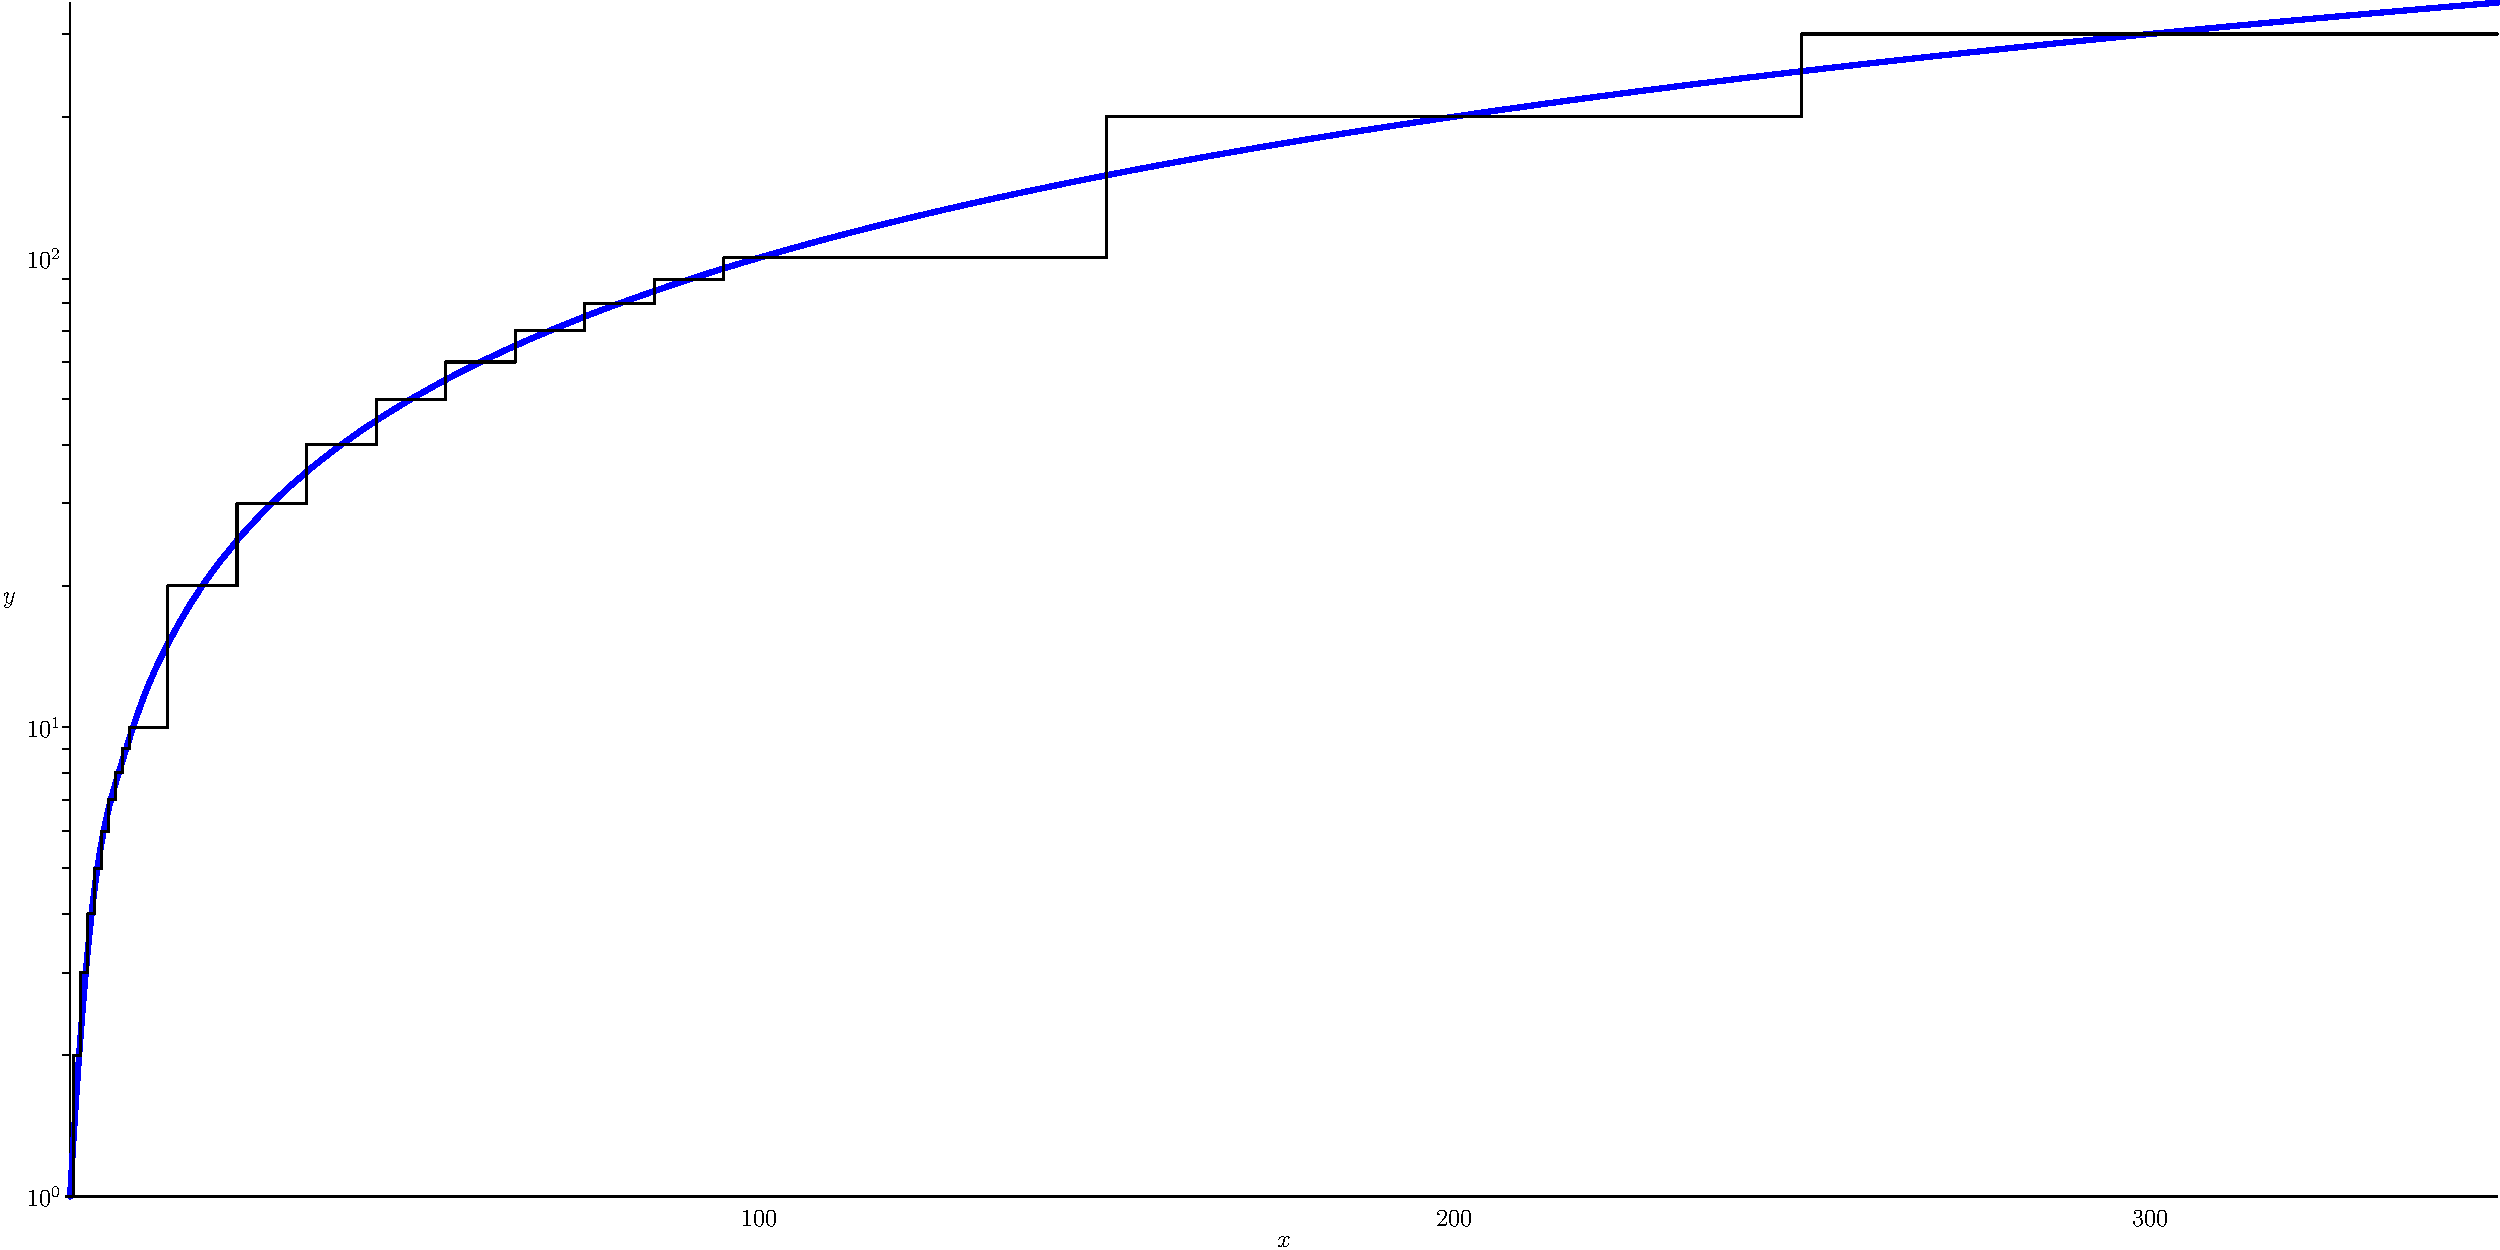
\includegraphics[width=0.5\textwidth]{chart}
  \caption{Illustration of ballpark figures versus actual figures, as a log chart.}
  \label{fig:ballpark}
\end{figure}

Given a (possibly very large) number, print its numerically closest
representation that has only one digit other than trailing zeroes.

The closeness of the representation $r$ of a number $n$ is defined by
$\text{abs}(r - n)$.

\section*{Input}

The input consists of:
\begin{itemize}
  \item one line with the positive integer $n$ ($1 \le n \le 10^{18}$).
\end{itemize}

\section*{Output}

Output the closest number to $n$ with exactly one significant (non-zero) figure.
If there are two equally-close answers, print the larger one.
